\documentclass[border=0.8ex,svgnames,tikz]{standalone}
\usepackage{amsmath,mathtools}
\usepackage{fontspec}
\setmainfont{Source Serif 4}
\setsansfont{Source Sans 3}
\setmonofont{Source Code Pro}
\usetikzlibrary{fit,chains}
\newcommand{\nodegen}[1]{
  \begin{scope}[
    start chain=going right,
    every node/.append style={join,on chain},
    every join/.style={->,>=latex},
    ]
    \node(build#1)[right of=path-#1]{build-#1};
    \node(test#1){test-#1};
    \node(deploy#1){deploy-#1};
  \end{scope}
}
\begin{document}
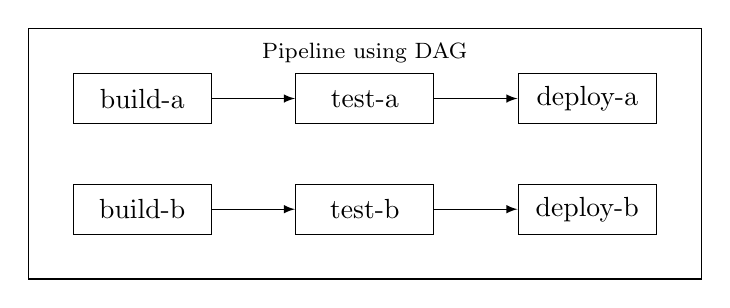
\begin{tikzpicture}[
  node distance=3em,
  every node/.style={draw,minimum width=5em,minimum height=1.8em},
  every path/.style={draw,>=latex},
  ]
  \coordinate(path-a) at (0,4em);
  \nodegen{a};
  \coordinate(path-b) at (0,0em);
  \nodegen{b};
  \node[fit=(builda)(deployb),draw,inner sep=1.6em,
  label={[yshift=-1.8em]above:{\footnotesize Pipeline using DAG}}]{};
\end{tikzpicture}
\end{document}
